\section{Newsfeed App - Recherchebericht}
\label{section:realisation:newsfeed_app}

\subsection{Lastenheft}
\begin{itemize}
\item Es ist ein Recherchebericht zu erstellen, der sich mit Produkten, Lösungen und Anwendungen (im Folgenden als Anwendungen zusammengefasst) befasst. Konkret geht es um Anwendungen, die es Unternehmen ermöglichen, ihre Mitarbeiter über unternehmensinterne Vorgänge zu informieren und den Mitarbeitern eine Interaktion mit dem Unternehmen ermöglichen. 
\item Der Bericht soll eine Übersicht über die am Markt etablierten Anwendungen liefern. Ein Fokus soll auf den Anreizen liegen, mit welchen die Anwendungen die Mitarbeiter zur Benutzung motivieren.
\item Des Weiteren soll im Bericht untersucht werden, welche Umfragefunktionalitäten in der jeweiligen Anwendung bereits existieren und wie diese potentiell durch PulseShift genutzt werden könnten. 
\item Darüber hinaus soll der Bericht aufzeigen, welche weiteren Möglichkeiten zur Einbindung einer Umfrage durch PulseShift es jeweils gibt und wie flexibel diese Möglichkeiten genutzt werden können.
\item Außerdem sollen in dem Bericht die Erfahrungen von Referenzkunden, die die Anwendung bei Offline-Mitarbeitern einsetzen, beschrieben werden. 
\item Sofern jeweils eine Preisstruktur verfügbar ist, soll außerdem auf diese eingegangen werden.
\end{itemize}

\subsection{Pflichtenheft}
\begin{itemize}
\item Es wird ein Recherchebericht erstellt, der sich mit Produkten, Lösungen und Anwendungen (im Folgenden als Anwendungen zusammengefasst) befasst. Konkret wird es um Anwendungen gehen, die es Unternehmen ermöglichen, ihre Mitarbeiter über unternehmensinterne Vorgänge zu informieren und den Mitarbeitern eine Interaktion mit dem Unternehmen ermöglichen.
\item Der Bericht wird eine Übersicht über die am Markt etablierten Anwendungen liefern. Für die Marktführer wird herausgearbeitet, mit welchen Anreizen sie die Mitarbeiter zur Benutzung der Anwendung motivieren. Sofern jeweils möglich werden die Anwendungen dazu neben einer Internetrecherche auch aktiv getestet.
\item Des Weiteren werden im Bericht die Möglichkeiten zur Integration der Umfrage von PulseShift in die jeweilige Anwendung aufgezeigt. Diese wird tabellarisch mit zusätzlichen erläuternden Texten gegenübergestellt. Dabei wird sofern jeweils verfügbar sowohl auf die Umfragefunktionalitäten der Anwendung als auch das Abspringen zur Umfragefunktion von PulseShift eingegangen. Außerdem werden jeweils mögliche weitere anwendungsspezifische Möglichkeiten wie beispielsweise ein Einbinden der Umfrage mittels iFrame vorgestellt.
\item Abschließend werden die Erfahrungen von Referenzkunden dargelegt. Dabei wird der Fokus auf Erfahrungen liegen, die im unmittelbaren Zusammenhang mit dem Einsatz bei Offline-Mitarbeitern stehen.
\item Der Bericht wird innerhalb des Projektabschlussberichts in Latex erstellt.
\end{itemize}


\subsection{Firstline Worker}

Die Firstline Workforce klassifiziert alle Mitarbeiter ohne festen Computer-Arbeits\-platz. Sie repräsentieren die mehr als zwei Milliarden Menschen  in Rollen, die sie zum ersten Kontaktpunkt zwischen einem Unternehmen und der Außenwelt machen. Sie sind die Menschen hinter der Theke, am Telefon, in den Kliniken und in der Werkstatt. Sie bilden das Rückgrat vieler der weltweit größten Branchen - Einzelhandel, Restaurants, Gastgewerbe, Reisen, Fertigung und Bauwesen. In dieser Rolle sind sie oft die ersten, die Kunden ansprechen, die ersten, die die Marke eines Unternehmens repräsentieren und die ersten, die Produkte und Dienstleistungen in Aktion sehen.


\begin{figure}[H] 
\centering 
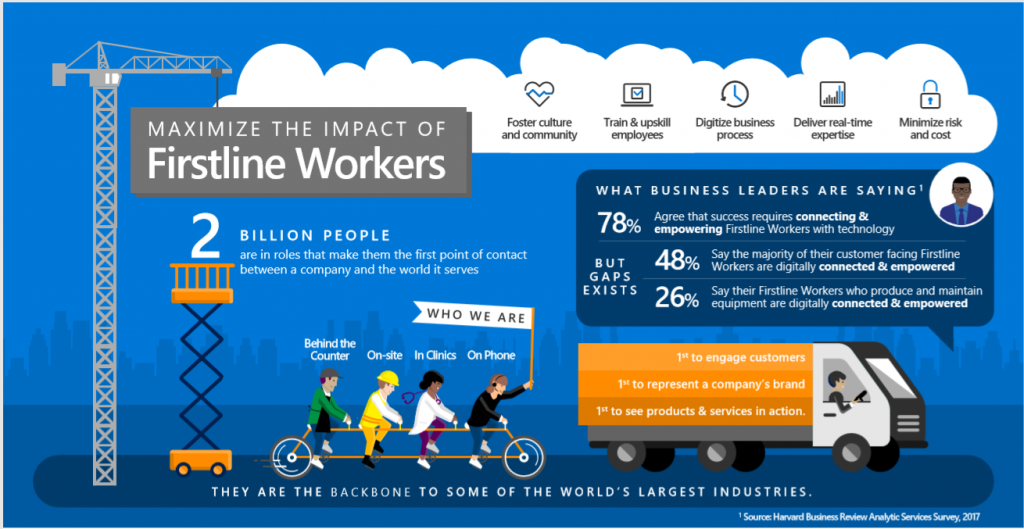
\includegraphics[scale=0.48]{images/frontlineworkers} 
\caption[Frontline Workers]{Firstline workers Aufgabenbereiche\protect} 
\label{dem} 
\end{figure}


\subsection{Microsoft StaffHub}

Microsoft StaffHub ist eine speziell für die Firstline Workforce in Office 365 entwickelte App. Es wurde speziell entwickelt, um die Fähigkeiten, Werkzeuge und Informationen zu liefern, die Firstline Mitarbeiter benötigen, um effektiv zu arbeiten und Spitzenleistungen zu erbringen. Dieser Service kombiniert Terminplanung, Aufgabenverwaltung, Dokumente, Personen und Tools an einem sicheren Ort - mit der Möglichkeit, sich mit anderen arbeitsbezogenen Apps und Ressourcen zu verbinden.
\begin{itemize}
\item Zugriff auf Schichtplan
\item Kommunikation innerhalb des Teams
\item Zugriff auf wichtige Information übers Handy
\item Manager können Schichtplan bearbeiten und Informationen verbreiten
\end{itemize}

\subsubsection{Verfügbarkeit}
Microsoft StaffHub ist derzeit verfügbar im Web, iOS und Android. Momentan ist StaffHub nicht als eigenständiges Projekt, sondern nur im Rahmen der folgenden Office 365-Geschäftspläne verfügbar: F 1, E1, E3 und E5. Wenn ein Kunde bereits einen dieser Pläne hat, kann er direkt Microsoft StaffHub verwenden. Der Einstieg ist ganz einfach. Erstanmelder können sich mit ihrem Office-365 Arbeitskonto unter http://staffhub.office.com anmelden. Von dort aus können sie Zeitpläne für ihre Teams erstellen und verwalten, wichtige Ressourcen und Unternehmensnachrichten hochladen und teilen sowie Firstline Workers einladen, die Anwendung herunterzuladen.

\subsubsection{Schedule \& Task Management}
Das Schedule \& Task Management ermöglicht es dem Manager, die Schichten für die Mitarbeiter zuzuweisen, zu aktualisieren und allgemein zu verwalten. Die Mitarbeiter können gleichzeitig untereinander Schichten tauschen und Urlaub beantragen, während der Manager stets die komplette Übersicht und Kontrolle bei Änderungen beibehält. 

\begin{figure}[H] 
\centering 
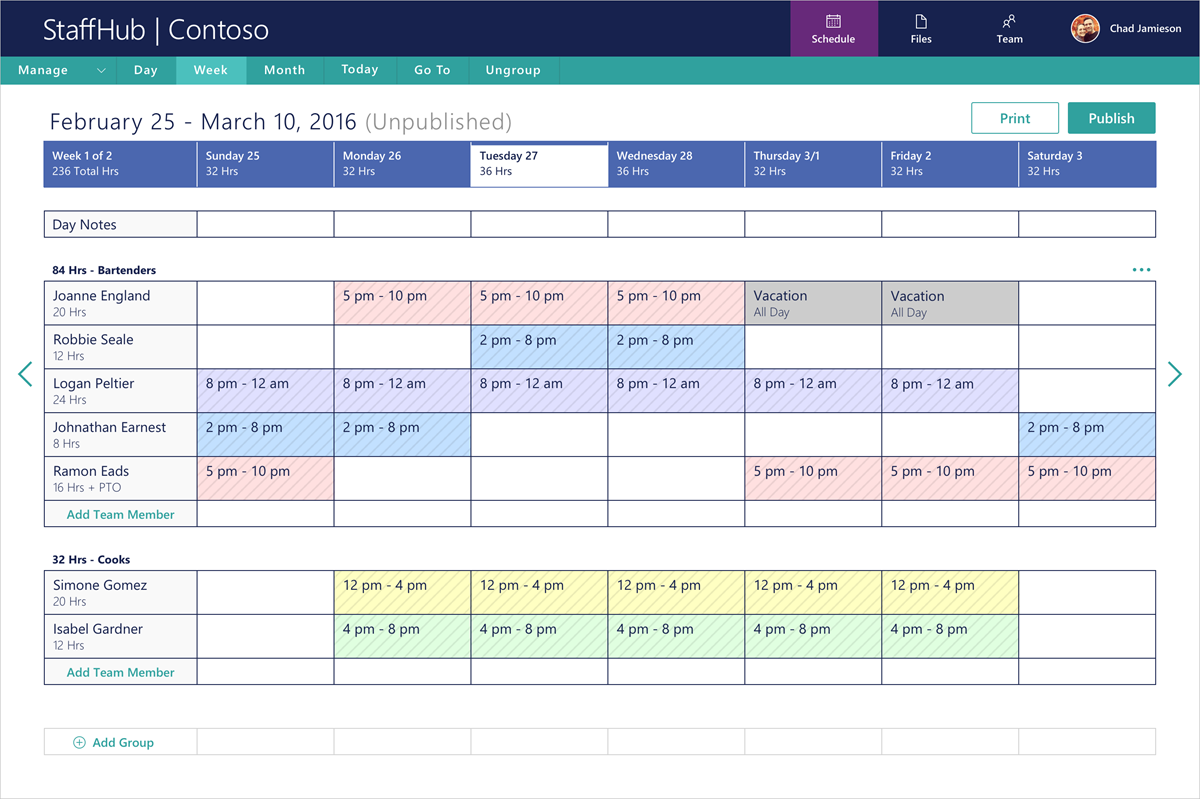
\includegraphics[scale=0.48]{images/schedule} 
\caption[Webansicht Schichtpläne]{Webansicht Schichtpläne\protect} 
\label{ws} 
\end{figure}

\begin{figure}[H] 
\centering 
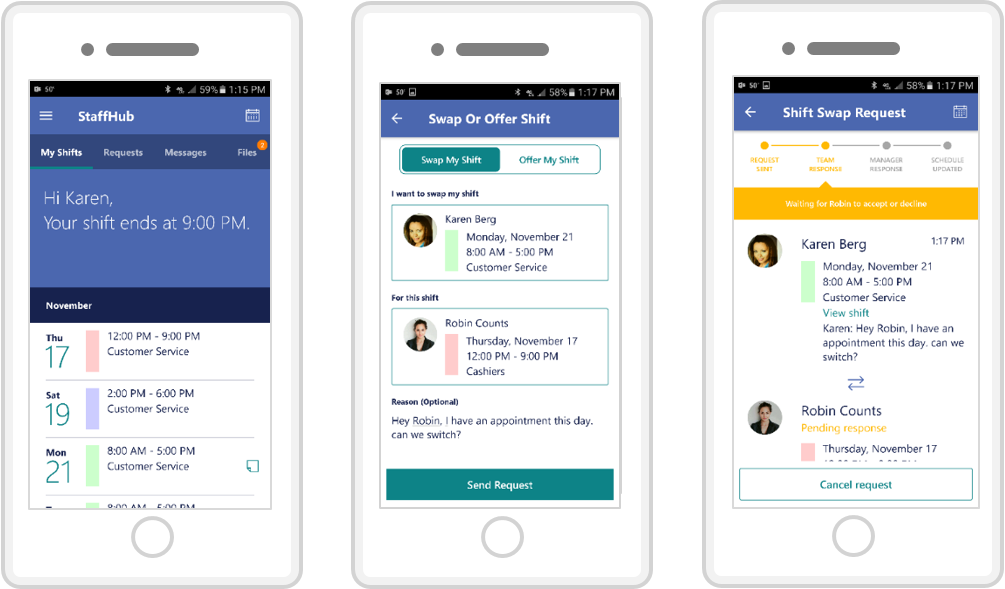
\includegraphics[scale=0.48]{images/schedulemobile} 
\caption[Schichtpläne tauschen mit dem Handy]{Schichtpläne tauschen mit dem Handy\protect} 
\label{ws} 
\end{figure}

Außerdem können einzelne Aufgaben und To-Dos gepflegt werden. Diese können direkt durch den Manager vergeben oder vom Mitarbeiter als Erinnerung für sich selbst angelegt werden. 

\begin{figure}[H] 
\centering 
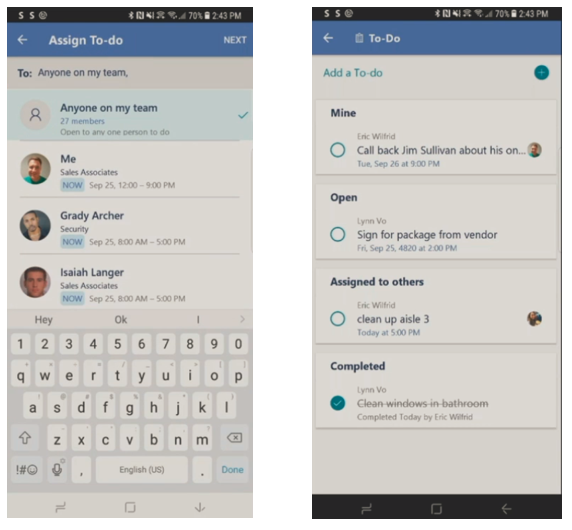
\includegraphics[scale=0.78]{images/todolist} 
\caption[To-Do Liste pflegen]{To-Do Liste pflegen\protect} 
\label{ws} 
\end{figure}

Für die Zukunft ist außerdem geplant, mithilfe der App eine Zeiterfassung in Realtime zu ermöglichen, sodass nicht mehr klassisch gestempelt werden muss.
Zusätzlich ist es möglich die Funktionalitäten zu erweitern und weitere Services und Apps an StaffHub anzubinden. Zusätzlich ist es möglich die Funktionalitäten zu erweitern und weitere Services und Apps an StaffHub anzubinden.

\subsubsection{Communications \& Community}

In StaffHub können jederzeit neue Kommunikationskanäle aufgesetzt werden, wodurch es möglich ist, Gruppen oder persönliche Chats zu starten. Des Weiteren können vom Unternehmen Best Practices oder Neuigkeiten in Form von Announcements unmittelbar an den Mitarbeiter kommuniziert werden.

\begin{figure}[H] 
\centering 
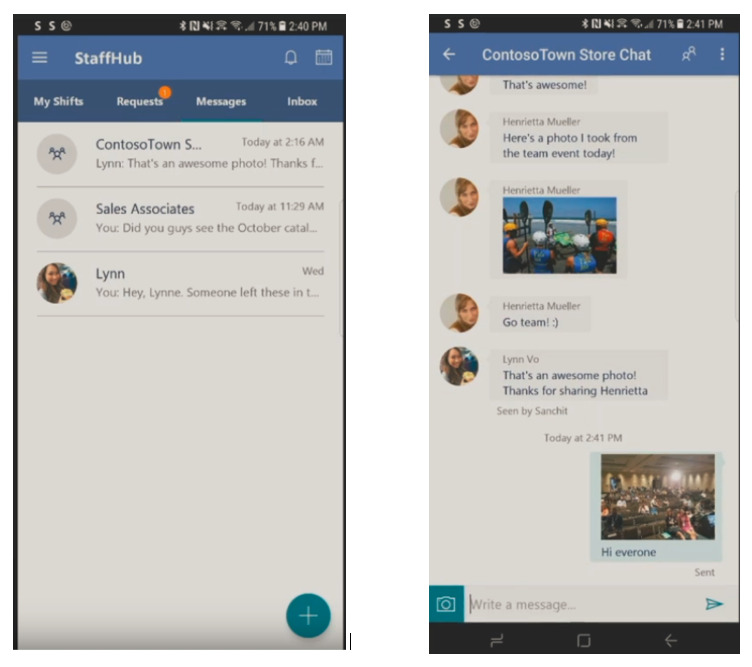
\includegraphics[scale=0.78]{images/groupchat} 
\caption[Teamchats]{Teamchats\protect} 
\label{ws} 
\end{figure}

\subsubsection{Training \& Onboarding}

Mit StaffHub ist es möglich Dokumente und Dateien zu verwalten und innerhalb des Unternehmens zu teilen. Dies wird unter anderem durch die Integration von SharePoint und Team Sites unterstützt. Auf den Inhalt kann man dabei direkt innerhalb der App zugreifen und dadurch Training und Onboarding-Aktivitäten planen.

\begin{figure}[H] 
\centering 
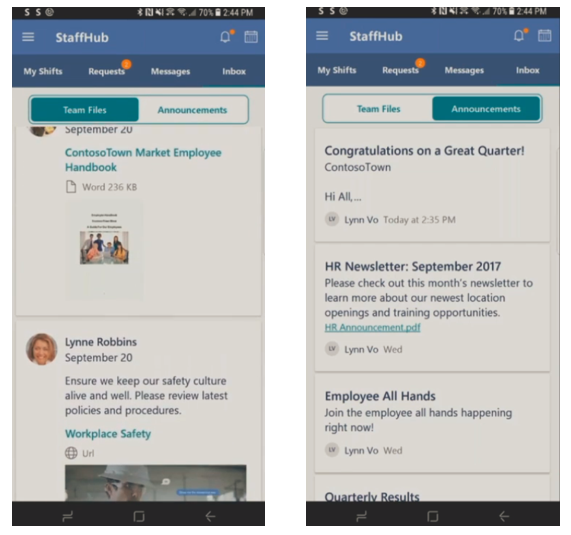
\includegraphics[scale=0.78]{images/communication} 
\caption[File Sharing und Announcements]{File Sharing und Announcements\protect} 
\label{ws} 
\end{figure}

\subsubsection{Identity \& Access Management}

StaffHub ermöglicht die Vergabe von Identitäten mit Hilfe von nur einer Telefonnummer. Eine Email-Adresse ist in diesem Fall optional. Die einzelnen User können dabei zentral mit Office 365 verwaltet werden.

\begin{figure}[H] 
\centering 
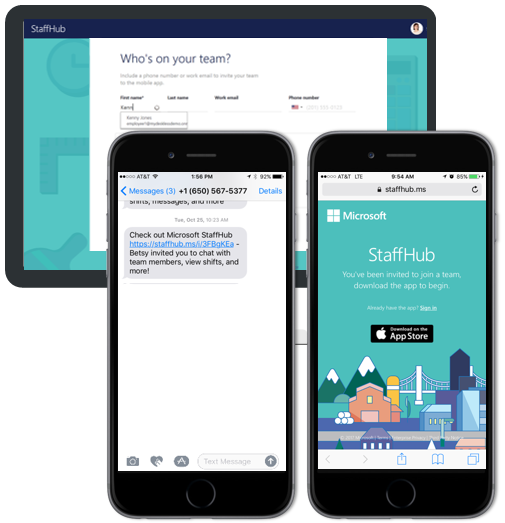
\includegraphics[scale=0.82]{images/invite} 
\caption[Telefonnummer statt E-Mail zur Identifikation]{Telefonnummer statt E-Mail zur Identifikation\protect} 
\label{ws} 
\end{figure}

\subsubsection{API \& Business Integration}

In StaffHub können über die API 3rd Party Lösungen für Workforce Management eingebunden werden. Des Weiteren kann man benutzerspezifische Integration für interne Applikationen und Prozesse hinzufügen. Zusätzlich ist die Integration mit Kronos WorkForce Central V8 unterstützt und es werden Connectors bereitgestellt, um mit Microsoft Flow zu arbeiten.
Die API ist nach eigenen Angaben zunächst nur als private Vorschau verfügbar. Jedoch ist eine Erweiterung der API in naher Zukunft geplant und bei weiteren Integrationen und möglichen Partnerschaften kann man sich direkt an staffhubinfo@microsoft.com wenden. Die APIs soll nach einigen Tests und Optimierungen der Öffentlichkeit kostenlos zur Verfügung gestellt werden.

\begin{figure}[H] 
\centering 
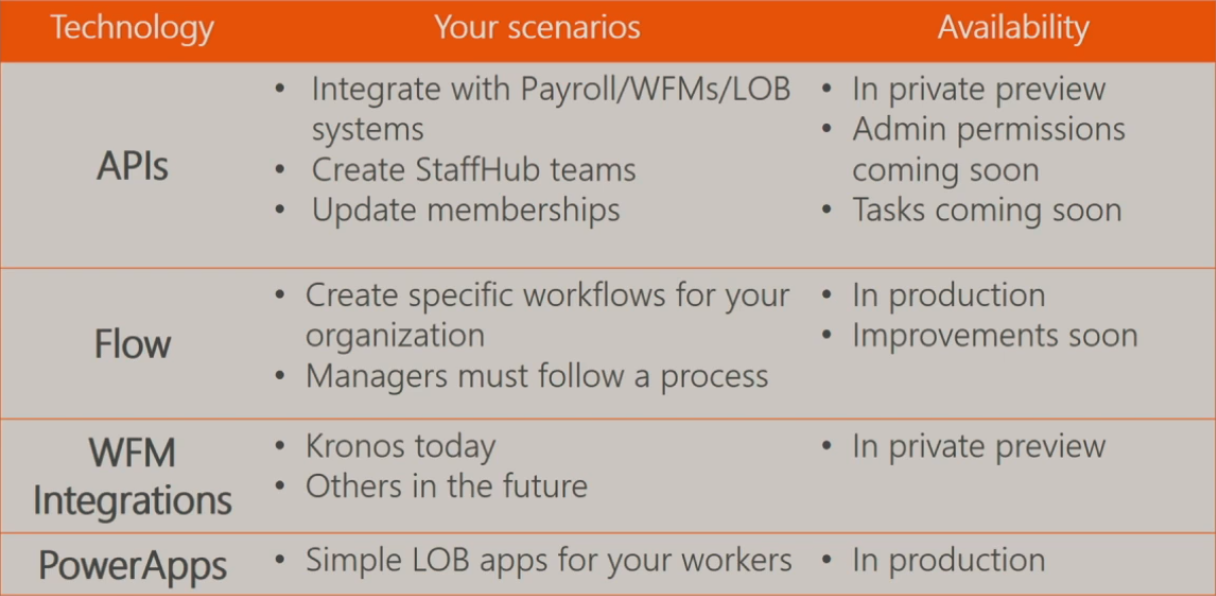
\includegraphics[scale=0.42]{images/msapi} 
\caption[Cheat Sheet über Schnittstellen]{Cheat Sheet über Schnittstellen\protect} 
\label{ws} 
\end{figure}

\subsubsection{Unterschied zu Microsoft Teams}
Microsoft Teams ist ein Chat-basierter Arbeitsbereich, der Personen, Unterhaltungen und Inhalte zusammenführt. Microsoft StaffHub ist hingenen eine speziell entwickelte App für die Firstline Workforce zur Verwaltung ihres Arbeitstages. Laut Microsoft ist die Kommunikation für beide wichtig und kündigten kürzlich die Integration von StaffHub Messaging und Microsoft Teams an, um es Firstline Workers zu ermöglichen, sich mit allen Mitarbeitern zu verbinden und zusammenzuarbeiten.

\subsubsection{Referenzkunden}
Bisher haben folgende Unternehmen Microsoft StaffHub im Einsatz: 

\begin{itemize}
\item Accor Hotels (240.000 Mitarbeiter, 200.000 Firstline Workers, 95 Länder)
\item VCA Animal Hospitals (800+ Standorte, 250.000 Mitarbeiter)
\end{itemize}
 
\subsubsection{Bewertung}
Insgesamt erweist sich Microsoft StaffHub als sehr umfrangreiches und mächtiges Tool, obwohl es erst vor kurzem für die Öffentlichkeit verfügbar ist. Dadurch besteht die Möglichkeit, dass PulseShift sich die Funktionen von StaffHub zu Nutze machen und die Umfrage in das Tool einbinden kann. Dafür gibt es mehrere Optionen: PulseShift kann ein eigenen User beantragen und ist neben allen Mitarbeitern innerhalb des nutzenden Unternehmens zusätzlich als Drittpartei eingebunden. Dies ermöglicht, dass PulseShift in einem Teamchat regelmäßig auf die Umfrage aufmerksam machen kann oder die Umfrage zentral an alle Mitarbeiter über ein Announcement verteilen, da es problemlos möglich ist einen Link oder ein Dokument innerhalb der App aufzurufen. Außerdem kann es jedem Nutzer individuell als To-Do Task assigned werden, wodurch sich der Mitarbeiter eher in der Verpflichtung sieht diese Aufgabe auch abzuhaken.
Darüber hinaus besteht mit der API, die in Zukunft weiter ausgebaut wird, die Möglichkeit die Umfrage von außen über eine Schnittstelle in die Applikation einzubinden.

\subsection{Inkling}
Inkling ist eine mobile Plattform, die die Mitarbeiter des Unternehmens an vorderster Front verbindet und ihnen dabei hilft, ihr volles Potenzial auszuschöpfen. Der Fokus liegt dabei auf den Einzelhandel.

Mit Inkling Collaboration erzielt man eine bessere Ausführung, indem die Frontline mit den benötigten Mitarbeitern und Ressourcen verbunden wird. Store-Teams verbringen weniger Zeit im Backoffice und mehr Zeit auf der Verkaufsfläche. Das bedeutet engagierte Mitarbeiter, zufriedenere Kunden und schnelleres Umsatzwachstum. 

\begin{figure}[H] 
\centering 
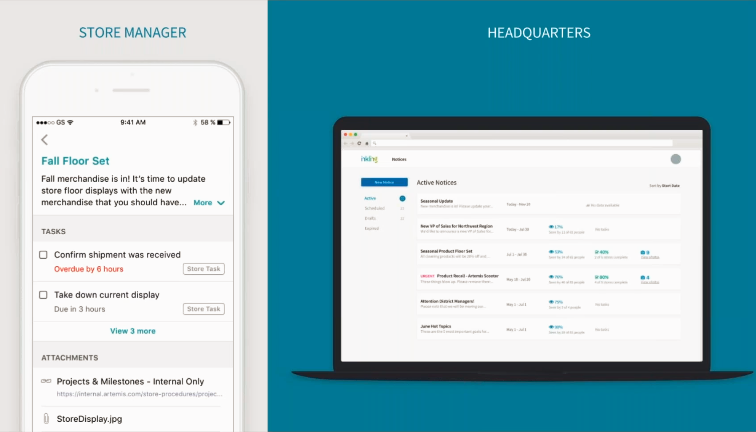
\includegraphics[scale=0.72]{images/inkgeneral} 
\caption[Überblick Inkling]{Überblick Inkling\protect} 
\label{ws} 
\end{figure}

\subsubsection{Taskmanagement}

Mit Inkling kann ein integrierter Satz von Prioritäten und Ressourcen verteilt werden, um die Produktivität zu steigern und die verbrachte Zeit der Mitarbeiter auf der Verkaufsfläche zu maximieren. Sobald eine neue Aufgabe einem Mitarbeiter zugeordnet wird, erhält dieser eine Benachrichtigung auf seinem Handy. In der App selbst hat der Mitarbeiter einen Überblick über alle Aufgaben mit entsprechender Priorisierung.

\begin{figure}[H] 
\centering 
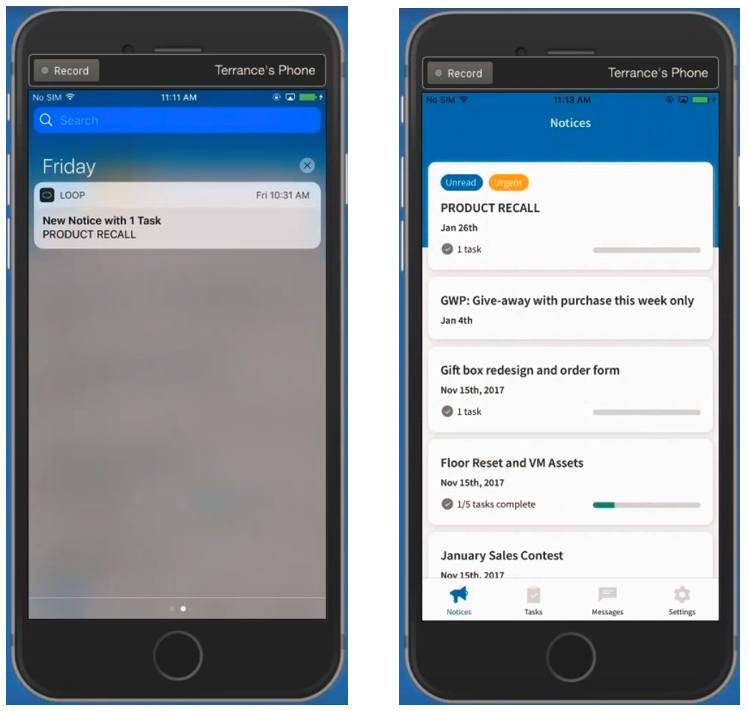
\includegraphics[scale=0.72]{images/inktasks} 
\caption[Aufgabenverwaltung]{Aufgabenverwaltung\protect} 
\label{ws} 
\end{figure}

Die einzelnen Aufgaben enthalten Detailbeschreibungen und können in Unteraufgaben eingeteilt werden und dabei Attachments beinhalten. Des Weiteren können Bilder genutzt werden, um die Vervollständigung einer Aufgabe zu bestätigen.

\begin{figure}[H] 
\centering 
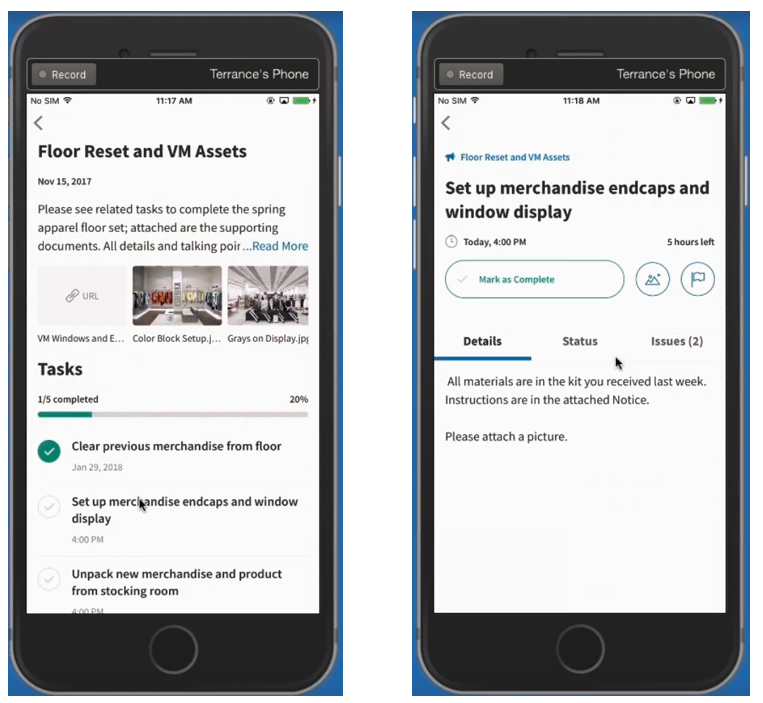
\includegraphics[scale=0.72]{images/inkdetails} 
\caption[Aufgaben im Detail]{Aufgaben im Detail\protect} 
\label{ws} 
\end{figure}

\subsubsection{Messaging}

Inkling Collaboration ermöglich sowohl Gruppen, als auch Einzelchats mit denen Bilder, Videos, Links und Dokumente geteilt werden können.

\begin{figure}[H] 
\centering 
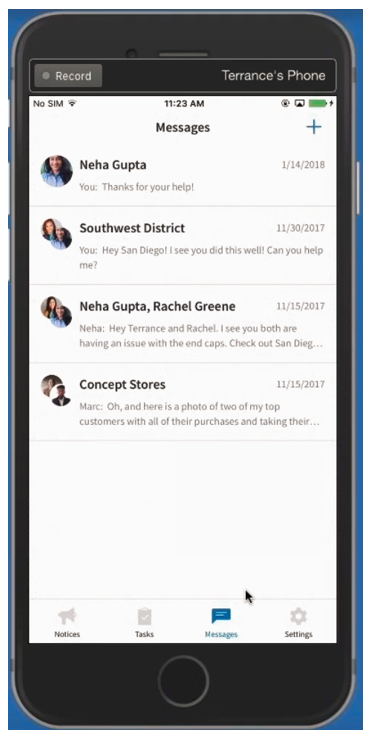
\includegraphics[scale=0.72]{images/inkmsg} 
\caption[Chats in Inkling]{Chats in Inkling\protect} 
\label{ws} 
\end{figure}


\subsubsection{Echtzeit-Analyse}

Die Daten und der momentane Prozess der Aufgaben aller Mitarbeiter kann jederzeit abgerufen und analysiert werden. Hierbei ist es möglich, den aktuellen Vervollständigungsgrad, hochgeladene Fotos und die Anzahl der Mitarbeiter, die die Aufgabe angesehen haben, einzusehen. 

\begin{figure}[H] 
\centering 
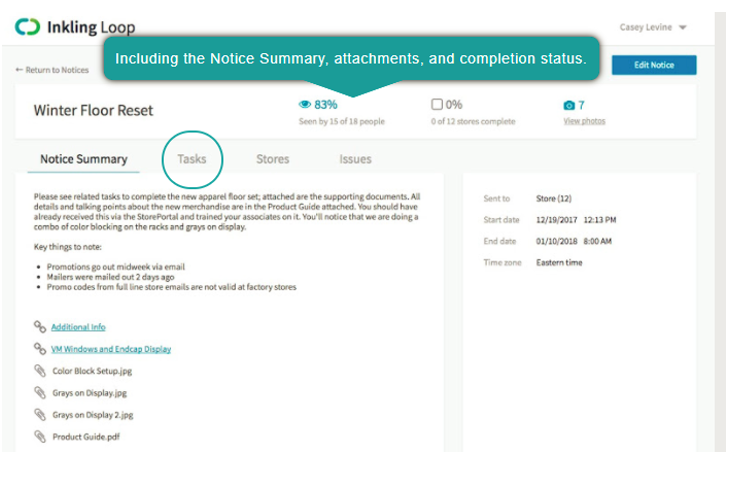
\includegraphics[scale=0.72]{images/inkweb} 
\caption[Webansicht über aktuelle Aufgaben]{Webansicht über aktuelle Aufgaben\protect} 
\label{ws} 
\end{figure}

\subsubsection{Referenzkunden}

Inkling wird von vielen bekannten Unternehmen wie McDonalds und Caterpillar genutzt. Ein Auszug wird in folgender Abbildung dargestellt:

\begin{figure}[H] 
\centering 
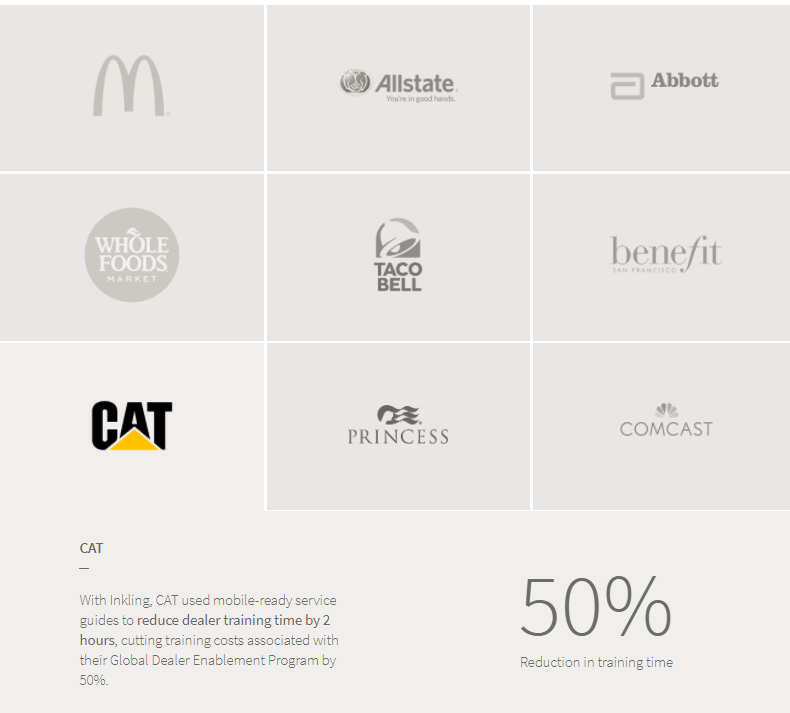
\includegraphics[scale=0.72]{images/inkcustomers} 
\caption[Übersicht Referenzkunden]{Übersicht Referenzkunden\protect} 
\label{ws} 
\end{figure}

\subsubsection{API}

Mit Inklings REST-API können ein Großteil der Funktionen der gehosteten Marktplatzlösung repliziert werden, um benutzerdefinierte Widgets und Börsenticker für das Intranet des Unternehmens zu erstellen, benutzerdefinierte Berichte zu erstellen, eine bestehenden Anwendung Handelsfunktionen hinzuzufügen oder einen eigenen benutzerdefinierten Marktplatz zu entwickeln. Die API von Inkling wird in Github verwaltet und kann nach entsprechender Absprache mit dem Unternehmen für einen Zugriff genutzt werden.

\subsubsection{Bewertung}

Insgesamt bietet Inkling viele Funktionalitäten, die gute Synergien mit der Umfrage von PulseShift ermöglichen können, wie beispielsweise die Funktion, mit der man einsehen kann, wie viele der Mitarbeiter die Umfrage bereits gesehen haben. Außerdem könnte man in Zukunft die Umfragen in Teilaufgaben unterteilen oder diese als solche in einer anderen Hauptaufgabe einbinden.
Jedoch liegt der Fokus bei Inkling letztendlich eindeutig auf dem Einzelhandelssektor. Daher ist die Applikation trotz einiger Synergien für die aktuelle Zielgruppe von PulseShift (Werksmitarbeiter) eher ungeeignet.



\subsection{Cotap}
Cotap ist eine von Zinc entwickelte mobile Nachrichtenapplikation für das Unternehmensumfeld. Sie ist insbesondere für \glqq Deskless\grqq Unternehmen geeignet. Es soll dem Unternehmen ermöglichen schnell und einfach mit seinen Mitarbeitern zu kommunizieren. 

Die Funktionalitäten der Applikation lassen sich in zwei Hauptkategorien aufteilen: 

\begin{itemize}
\item Kommunikationstools - zur Kommunikation im Unternehmen 
\item Analysetools - zur Analyse des Kommunikationsverhaltens und somit auch zur Analyse der Unternehmenssituation
\end{itemize}

Im Folgenden werden diese Tools, aufgegliedert in die einzelnen Funktionsbereiche, vorgestellt.

\subsubsection{Kommunikationstools}

\begin{itemize}
\item 1:1 Messages - senden von direkten Nachrichten an jeden aus der Organisation
\item Group Messages - um sich beispielsweise innerhalb einer Abteilung abzustimmen
\item Content Sharing - um Dokumente und weitere wichtige Informationen mit anderen Mitarbeiten zu teilen
\item Hands Free - Nachrichten werden laut vorgelesen und können eingesprochen werden
\item 3RD Party Messaging - Personen, die nicht der eigenen Organisation zugeordnet sind können einfach über die E-Mail-Adresse hinzugefügt werden
\item Push to Talk - Schnelle und einfache Benachrichtigung anderer Mitarbeiter oder Gruppen durch Walkie-Taklie-Funktion
\item Broadcast - zum Versenden dringender und wichtiger Nachrichten an alle Beteiligten, zusätzliche Funktionalität eines Pop-Ups
\end{itemize}

Die drei letzte Komponenten 3RD Party Messaging, Push to Talk und Broadcast können für unseren Use Case genutzt werden.

3RD Party Messaging kann es PulseShift ermöglichen, über einen Gruppenchat, in welchen sie eingeladen wurden, einen Link zur Umfrage zu posten. So könnten jeweils einzelne Abteilungen gezielt erreicht werden.

Durch Push to Talk kann darauf aufmerksam gemacht werden, dass es eine Umfrage gibt an der man teilnehmen kann. Hier ist es jedoch entscheidend, dass die Übertragung der Nachricht in Tonform und live ist. 

Mithilfe des Broadcasts könnte ein Link zur Umfrage versendet werden. So wird dem Mitarbeiter zusätzlich suggeriert, dass es wichtig ist an dieser Umfrage teilzunehmen. 

\subsubsection{Analysetools}
Mithilfe der Analysetools werden die gesendeten Nachrichten, hinsichtlich Menge, Inhalt, Länge und weiteren Kriterien analysiert, um weitere Informationen zu generieren. 

Die verschiedenen Analysen werden im Folgenden kurz dargestellt: 

\begin{itemize}
\item Analyse der einzelnen Kommunikationskanäle
\item Historischer Verlauf der Broadcasts
\item Analyse der Anzahl und Größe von gesendeten Nachrichten
\item Networkmap, um zu zeigen wer mit wem kommuniziert
\end{itemize}

Aus diesen Informationen könnte ein Mehrwert für die Umfragen geschlossen werden, dazu wäre jedoch eine komplette Erweiterung des Umfragekonzeptes notwendig und wird daher vorerst verworfen.

\subsubsection{Integrationsmöglichkeiten}
Cotap bietet die Möglichkeit, andere Apps zu integrieren, sodass der Nutzer die App nicht verlassen muss, um mit anderen Apps zu interagieren. Mithilfe dieser Funktionalität könnten die Umfragen von PulseShift sehr einfach eingebunden werden. 

Außerdem können automatische Benachrichtigungen erstellt werden, um die Mitarbeiter auf die Umfrage hinzuweisen.

\subsubsection{Kosten}
Die App Cotap kann zunächst einmal kostenlos im Playstore herunter geladen werden. Mit Hilfe dieser kostenlosen Version können unbegrenzt Nachrichten gesendet werden sowie Fotos, Videos und der eigene Standort geteilt werden. Außerdem sind Basic-Integrationen möglich. 

Für 5 Dollar monatlich ist es möglich, Audio- und Video-Anrufe bis zu 100 Minuten pro Nutzer pro Monat zu tätigen und Daten bis zu zwei GB pro User pro Monat zu versenden. In diesem Paket ist außerdem die Gruppenorganisation und Nutzung enthalten. Des Weiteren können individuelle Benachrichtigungen erstellt werden.

Das teuerste Paket ist für 10 Dollar pro Monat erhältlich. Hier können Audio- und Video-Anrufe bis zu 250 Minuten pro Nutzer pro Monat getätigt werden. Außerdem können unlimitiert Daten versendet und empfangen werden. Nun können Enterprise-Files sowie ein Single Sign-One integriert werden. Außerdem kann alles aktiv überwacht und die Analysetools somit genutzt werden.

\subsubsection{Bewertung}
Cotap erscheint als eine gute Möglichkeit, um die Umfragen von PulseShift zu integrieren. Die genaue Zusammenarbeit zwischen Cotap, PulseShift und dem jeweiligen Unternehmen muss jedoch abgeklärt und die genauen Kosten für den speziellen Fall ermittelt werden.
